% !TEX root = index.tex

\section{The Topology behind the Algebra}
\epigraph{It is my experience that proofs involving matrices can be shortened by 50\% if one throws the matrices out.}{E. Artin}

 Most problems in this section are (*) or harder and hence optional.

\begin{ques}
  Show that for a space $X$ if some good cover has dimension $n$ then $\check H^i(X) = 0$ for $i > n$.
\end{ques}

\begin{definition}
  The {\bf Euler characteristic} of a space $X$ is defined as
  \begin{align*}
    \chi(M) := \sum \limits_{i \in \Z} (-1)^i \dim \check H^i(X)  = \dim \check H^0(X) - \dim \check H^1(X) + \dim \check H^0(X) \pm \dots
  \end{align*}
\end{definition}

\begin{ques}
  Let $M$ be a $g$ holed torus.
  Triangulate $M$ and suppose there are $V$ number of vertices, $E$ number of edges, and $F$ number of faces in the triangulation. Find a good cover of $M$ using this triangulation and prove that
  \begin{align*}
    \chi(M) = V - E + F
  \end{align*} (Recall that we don't need to find the maps $d^i$ to find the Euler characteristic.)
\end{ques}

\begin{ques}
Let $G$ be a connected graph. Let $T$ be a maximal tree in $G$ i.e. $T$ is a subgraph of $G$ which is a tree such that adding any edge of $G$ to it creates a cycle. Find a cover $\U$ of $G$ containing $T$ as an element (i.e. $T \in \U$). Use this cover to find a topological interpretation of $\dim \check H^1(G)$.
\end{ques}


% \begin{ques}
%   By gluing the sides of a square in funky ways we can create the Klein Bottle and the Real Projective Plane. Find their Cech cohomologies. (We can find open covers for torus, Klein bottle, and projective plane containing exactly 3 sets.)
%   \begin{figure}[H]
%   	\centering
%     \begin{subfigure}[t]{0.3\textwidth}
%   		\centering
%   		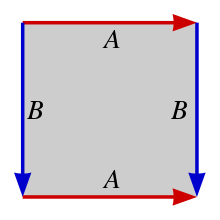
\includegraphics[height=2.5cm]{Torus}
%       \caption{Torus}
%   	\end{subfigure}
%     \begin{subfigure}[t]{0.3\textwidth}
%   		\centering
%   		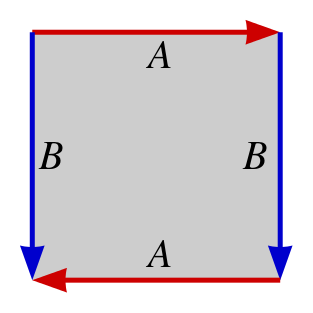
\includegraphics[height=2.5cm]{KleinBottle}
%       \caption{Klein Bottle}
%   	\end{subfigure}
%   	\begin{subfigure}[t]{0.3\textwidth}
%   		\centering
%   		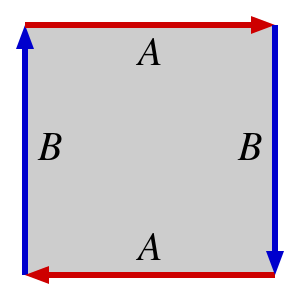
\includegraphics[height=2.5cm]{ProjectivePlane}
%       \caption{Projective Plane}
%   	\end{subfigure}
%   \end{figure}
% \end{ques}


We'll now find a topological interpretation for $\check H^0$. Let $X$ be a connected space with a good cover $\U = \{ U_1, U_2, \dots, U_n\}$. Assume that all the non-empty $U_i$ and $U_{\{i,j\}}$ are connected (this is simplify to our arguments, the proof works without this simplification). We have
\begin{align*}
  \L^0 &= \L(U_1) \oplus \L(U_2) \oplus \dots \oplus \L(U_n) \\
  \L^1 &= \L(U_{\{1,2\}}) \oplus \L(U_{\{1,3\}}) \oplus \dots \oplus \L(U_{\{n-1,n\}})
\end{align*}
and $\check H^0(X)$ is the kernel of the restriction maps $d^0 : \L^0 \rightarrow \L^1$. \begin{center}
  \begin{tabular}{ l | c c  }
        & $U_l$ & $\cdots$ \\\hline
    $U_{\{i,j\}}$ &   0 \mbox{ or } 1    &      \\
    \vdots &       &
  \end{tabular} $ = d^0$
\end{center}

\begin{ques} $ $
  \begin{enumerate}
    \item As $U_{\{i,j\}} = U_i \cap U_j$, argue that every row of the matrix $d^0$ (in the canonical bases) has exactly 2 non-zero entries.
    \item Argue that because $X$ is connected every open set in the cover $U_i$ must intersect some other $U_j$. What does this imply for the matrix $d^0$?
    \item Show that
    \begin{align*}
        \ker d^0 = \{ [0, 0, \dots, 0]^T, [1, 1, \dots, 1]^T\}
    \end{align*}
    and hence $\dim \check H^0(X) = 1$.
    \item Suppose $Y$ is another topological space.
      Find the Cech cohomologies of $X \sqcup Y$ (the disjoint union of $X$ and $Y$) in terms of  $X$ and $Y$. In particular, what is $\check H^0(X \sqcup Y)$?
    \item Find a topological interpretation of $\dim \check H^0(Z)$ for a general topological space $Z$ (not necessarily connected).
  \end{enumerate}
\end{ques}

\begin{ques} Find the Cech cohomologies of $X \vee Y$ in terms of  $X$ and $Y$. (Assume we have appropriate good covers.)
\end{ques}

\newpage
We'll next prove that $\R^n \not \cong \R^m$ (non-homeomorphic) if $n \not = m$. Let
\begin{align*}
  S^n &= \{ (x_0, x_1, \dots, x_n) \in \R^{n+1}: x_0^2 + x_1^2 + \dots + x_n^2 = 1 \}
\end{align*}
\begin{ques} $ $
  \begin{enumerate}
  \item Let $X, Y$ be topological spaces such that $Y$ is contractible. If $\U$ is a good cover for $X$, find a good cover for $X \times Y$. Show that $\check H^i(X) \cong \check H^i(X \times Y)$ for all $i \in \Z$. In particular, this is true when $Y = (0,1)$.
  \item Show that $\R^{n} \setminus \{ 0 \} \cong S^{n-1} \times (0,1)$.
  \item Let $X, Y$ be topological spaces. Show that if $X \cong Y$ then $\check H^i(X) \cong \check H^i(Y)$.
  \item Conclude that if $\R^n \cong \R^m$ then  $\check H^i (S^{n-1}) \cong \check H^i (S^{m-1})$ for all $i \in \Z$.
\end{enumerate}
\end{ques}
\noindent Thus we've reduced the problem to a cohomology computation, which we can do by finding an appropriate good cover of $S^{n}$. Let \begin{align*}
  S^n_+ &= \{ (x_0, x_1, \dots, x_n) \in \R^{n+1}: x_n \ge 0, x_0^2 + x_1^2 + \dots + x_n^2 = 1 \}\\
  S^n_- &= \{ (x_0, x_1, \dots, x_n) \in \R^{n+1}:  x_n \le 0, x_0^2 + x_1^2 + \dots + x_n^2 = 1 \}
\end{align*}


\begin{ques} $ $
\begin{enumerate}
  \item What is $S^0$?
  \item What are the dimensions of the Cech cohomologies of $S^0$, $S^1$, and $S^2$? Based on these make a guess as to what the dimensions of the Cech cohomologies of $S^n$ are.
\end{enumerate}
\end{ques}
\noindent We'll find the cohomologies of $S^n$ using induction.
For a non-empty subset $X \subseteq S^{n-1}$ define the (positive) cone over $X$, denoted $C_+ X$, to be a subspace of $S^{n}_+$ defined as
\begin{align*}
  C_+ X = \{ (tx_0, tx_1, \dots, tx_{n-1}, x_n) \in S^{n}_+ : t \in \R_{\ge 0}, (x_0, x_1, \dots, x_{n-1}) \in X \}
\end{align*}
Define the cone over the empty set $C_+(\phi)$ to be the single point $(0,\dots,0,1)$.

\begin{ques} Let $X,Y \subseteq S^{n-1}$.
\begin{enumerate}
  \item Let $X$ be some subset of $S^1$. Draw the cone $C_+X \subseteq S^2$.
  \item Prove that $C_+ X$ is connected and contractible.
  \item Prove that $C_+X \cap C_+ Y = C_+(X \cap Y)$ (this is why we need $C_+ \phi = (0,\dots,0,1)$).
  \item Prove that $C_+X \cap S^{n}_- \cong X$.
\end{enumerate}
\end{ques}
\begin{ques} By induction, suppose $S^{n-1}$ has a good cover $\U = \{ U_1, \dots, U_n\}$ with $n$ elements. (Check the base case.)
\begin{enumerate}
  \item  Prove that $\U' = \{ C_+ U_1, C_+ U_2, \dots, C_+ U_n, S^n_-\}$ is a good cover of $S^n$ (this proves the induction step).
  \item What is the dimension of this cover? Conclude that $\check H^{i}(S^n) = 0$ for $i > n$.
\end{enumerate}
\end{ques}
\noindent There are two types of intersections $\U'_I$:\\
$\qquad$ (type I) ones obtained by intersecting the sets $\{ C_+ U_1, C_+ U_2, \dots, C_+ U_n\}$  and \\$\qquad$ (type II) ones obtained by intersecting $S^n_-$ with the some of the sets from $\{ C_+ U_1, C_+ U_2, \dots, C_+ U_n\}$.
\begin{ques} $ $
  \begin{enumerate}
  \item Show that the intersections of type I are all contractible and the intersections of type II are the ones that show up in the Cech complex for $S^{n-1}$ and hence the Cech complex for $S^n$ contains a copy of the Cech complex of $S^{n-1}$ \emph{right} shifted by one.
  \item Use this to inductively prove that for $n \ge 1$
  \begin{align*}
    \check H^i(S^{n}) \cong \begin{cases}
      \F & \mbox{ for } i=0,n \\
      0 & \mbox{ otherwise }
  \end{cases}
  \end{align*}
  \item Conclude that $S^n \not \cong S^m$ and $\R^n \not \cong \R^m$ if $n \neq m$.
\end{enumerate}
\end{ques}
